% Capítulo 2
\chapter{Theoretical Background}

This chapter discusses factors related to Ubiquitous Computing, Cloud Computing and the technologies derived from them, as well as Ubiquitous and Smart Surveillance.

\section{Smart Cities}
Smart Cities is a significant paradigm for proposing and deploying various innovative technologies to make cities smarter and improve people's quality of life\cite{Pribyl2015}. The evolution of the Smart City concept is shaped by a complex mix of technologies, social and economic factors, governance arrangements, and policy and business drivers. The implementation of the Smart City concept, thus follows various paths depending on each city's specific policies, objectives, funding and scope. 
According to \cite{Schaffers2011}:

\begin{quotation}
\textit{"...\\A city may be called "Smart" when investments in human and social capital and traditional and modern communication infrastructure fuel sustainable economic growth and a high quality of life, with a wise management of natural resources, through participatory governance."\\...}
\end{quotation}

On the basis of cited definitions of smart cities, a set of factors can be enumerated that comprise the activities of autonomous, independent and aware citizens. In Figure \ref{fig:smart} the correlated features of smart cities are shown, which underlie the "smart" combination of endowments and activities of autonomous, independent and aware citizens.


\begin{figure}[htb!]
  \centering
    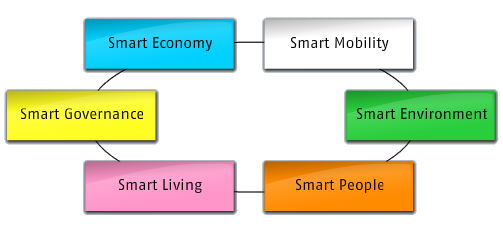
\includegraphics[scale=0.99]{Imagens/cap2_smarcite.png}
    \caption{Characteristics of Smart cities.}
    \label{fig:smart}
\end{figure}


Smart Mobility is a key feature in this proposal since its principles include "Sustainable, innovative and safe transport systems".
The availability of a secure, efficient and affordable transport system is one of the defining goals of any smart city. However, many cities today are facing challenges when implementing comprehensive "smart mobility" programs, including those that are secure and deal with a legacy infrastructure. The proposal outlined in this study was designed to improve the prospects of Smart Mobility.

\section{Ubiquitous Computing}

The constant technical advances in communication and computing have given rise to a scenario which a short time ago was only just being glimpsed by Pervasive Computing, and this means that computing is now a common feature of people's routine activities, and before long will form a part of our everyday lives. Furthermore, forecasts predict that microprocessors will become smaller and smaller and will soon be cheap enough to be embedded in digital devices, electronic appliances, everyday objects and clothes, as well as in cars.

This scenario is regarded as the new paradigm of the Century\cite{943998} \cite{Saha2003}  or the third wave of computing. It is enabling the physical world to be combined with the world of information and provides a wide range of services and ubiquitous applications such as target users, machines, data, applications, and various objects in physical space, so that they can interact with each other in a transparent way \cite{Ranganathan2005}. 

Hence, technology is gradually moving toward a world of ubiquitous computing, or incrementally having to rely on a set of heterogeneous devices to support a growing range of applications that are suited to this scenario.
According to its creator Mark Weiser, \textit{"deeper technologies are those that disappear"} \cite{Weiser1999}. From this perspective, Ubiquitous Computing is seeking to include computing in the physical world of the user, by allowing it to concentrate on the tasks that have to be accomplished and not just the tools that are needed for this.

According to \cite{Hansmann2001} ubiquitous systems are based on at least five principles:
\begin{itemize}

\item Diversity: This characteristic is related to devices, especially different kinds of computers in terms of specific task performance. For example, while a tablet is the most suitable device for viewing content, a notebook might be more appropriate for writing long texts;

\item Connectivity: The presence of different devices performing specific tasks, requires a high connectivity, to maintain cooperation and mobility among its users;

\item Decentralization: Despite the presence of servers, cooperative and distributed environments require decentralization, and it is worth noting that a flow of information is needed to be transmitted to the hosts, regardless of the particular characteristics of the environmental devices. Decentralization and diversity are accompanied by information synchronization, since it is essential for this system to be regularly updated in all the devices to maintain data consistency;

\item Invisibility: This supports the idea that technology in particular is a part of the environment. Computers offer a good means of achieving this and can become essential tools for interpreting our activities, since they are spread throughout the environment and have become present and imperceptible;

\item Context Awareness: ubiquitous applications must act in a desired context or situation that is chosen by the user so that they can become transparent. Applications provide their best performance when the users can understand the context in which they live and act on this information;

\item Proactivity: the ubiquitous software must be programmed to predict events and react without human interaction. 
\end{itemize}
Moreover, it is important to ensure that they do not take action on the basis of misinformation.
Although there have been numerous attempts to develop ubiquitous applications, the question of their practicality is still an open question, but this is not a major issue and beyond the scope of this work. On the basis of these principles, the concept of Ubiquitous Surveillance arises \cite{Orwel42} as a sub-area of Ubiquitous Computing that is concerned with surveillance. This work envisions that Ubiquitous Computing concepts should mainly provide invisibility, decentralization and connectivity among other benefits.


\section{Ubiquitous Surveillance}

Given the complexity of the features of Ubiquitous Computing, Ubiquitous Surveillance is a science that is geared towards monitoring citizens for their personal safety, and can also be applied in the area of public health, for example, to control epidemics, as well as in the fight against terrorism. This is achieved by obtaining valuable information from fixed cameras in public places or even micro air vehicles that operate in a semi-autonomous manner, as shown in \cite{Nardi2006}.

Among important studies that have put forward suggestions for improvements in ubiquitous surveillance systems, the work of \cite{Chen2009} should be mentioned. In this, the authors designed a multicast overlay in IP (Internet Protocol) networks, which offers the prospect of not only increasing the stability of ubiquitous surveillance services, but also providing a dynamic load balancing, since there is a wide bandwidth for end-user applications. Apart from making technical improvements, the work proposed by \cite{Wang2008}, applies an encryption algorithm to ensure the information security and privacy of those involved.

This and other proposals have focused on the evolution of image acquisition techniques in IP networks; however, they leave video analysis to the end-user, which means they are ubiquitous monitoring systems that are completely dependent on repetitive human endeavor. This fact makes them unviable for current surveillance systems, first because of the vast amount of data generated by the wide range of devices and second on account of the limited number of professional security experts that have the necessary skills to predict and detect these events. Moreover, the quality of life falls exponentially as these specialists have to be aware of multiple simultaneous monitoring systems throughout the working day.


\section{Smart Surveillance}

With regard to disability surveillance which is currently only carried out by human means, there are several research papers aimed at automating  ubiquitous surveillance  Some of them are listed in \cite{Sodemann2012}.  These works essentially use all the features combined with extraction techniques for machine learning and these are either Supervised or Unsupervised. Figure 5 shows a diagram of the intelligent monitoring targets and their interrelationship.

Thus the assumptions made about effective automatic surveillance are formed on the basis of a particular target environment. With the aid of this concept, the purpose of this study is to create a mechanism able to support smart surveillance algorithms by providing ubiquitous access, augmented processing power and seamless operations. Thus the analysis can show the objects used for these criminal acts.


\begin{figure}[htb!]
  \centering
    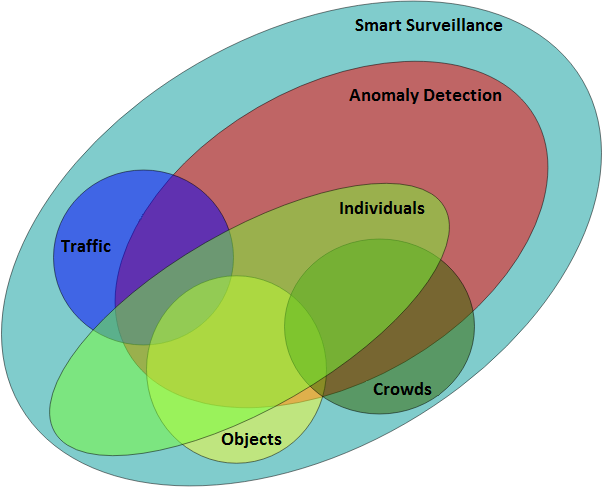
\includegraphics[scale=0.50]{Imagens/cap2_diagram.png}
    \caption{Venn Diagram - Smart Surveillance Targets.}
    \label{fig:targets}
\end{figure}

The formulation of an automated monitoring approach requires a starting- point that provides definitions and assumptions about the application being targeted. In the case of the proposal in question, making these assumptions is not an easy task because it entails a shifting environment and also the crimes may be committed in different ways. However, crimes committed in the vehicular environment are generally carried out with threatening weapons. In view of this, there are three measures that can be taken to make smart surveillance more effective, which are as follows: 

\begin{itemize}
\item Look for  dangerous objects in the environment, since they  are  less often found  than normal objects;
\item Be aware that  dangerous objects have significant features that make them  different  from normal objects;
\item Note that any particular objects that  appear on the scene may have some meaning. For example, if someone waves a gun in a bus, it can be assumed that a crime is bound to take place.
\end{itemize}

These measures make it clear how the tool should be employed. This is through video streaming which can benefit intelligent surveillance applications.


\section{Cloud Computing}

The concept of cloud computing has emerged from the need to allocate computing resources dynamically, and makes it possible to centralize scalable and secure processing, with sufficient momentum to support various types of applications. Vehicular applications can meet these requirements since they include even more dynamic environments. 
According to \cite{Buyya2009}:

\begin{quotation}
\textit{"...\\Cloud is a type of parallel and distributed system consisting of a collection of interconnected and virtualized computers that are dynamically provisioned and presented as one or more unified computing resource(s) based on service-level agreements established through negotiation between the service provider and consumers.\\..."}
\end{quotation}


On the basis of this definition, Cloud Computing technologies are adopted in this work to increase its processing power, seamless operations and ubiquitous access. All of its known benefits and characteristics will be described below in the next sub sections.

\subsection{Cloud Components}

The three main components of cloud computing are Clients, Data Center and Distributed Servers\cite{Velte2009}.
Clients are the devices with which end-users interact to manage their information on the cloud. Clients might be smart phones or computers without a hard disk (a thin client) or a regular computer (a thick client). A thin client is generally a web browser like Google's Chrome or Mozilla's Firefox. 

A Data Center is a collection of servers that contains the application subscribed by the customers who can access it via the Internet. Many virtual machines can execute tasks simultaneously on a single physical server, also known as the host. The number of virtual servers that can exist on a physical place depends on its size and speed and what applications will be running on the virtual server \cite{Velte2009}. 

The servers are placed in geographically dispersed locations so that they can provide available servers that are more reliable(Distributed Servers). This means that if one server fails, the service can be continued by another. They also increase scalability. If the cloud needs more hardware, it is not essential to deploy more servers only in the data center. They can be added at another site or be simply made a part of the cloud \cite{Velte2009}.

\subsection{Features of Cloud Computing}

According to the National Institute of Standards and Technology - NIST, there are five essential characteristics for cloud computing\footnote[8]{http://www.nist.gov/}. Each is described below in simple terms:

\begin{itemize}

\item Measured Service: Cloud Services are controlled and monitored by the cloud provider. This is crucial for billing, access control, resource optimization, capacity planning and other tasks;

\item On-Demand-Self-Service: The consumer can use cloud services as needed without any human interaction with the cloud provider; 

\item Ubiquitous Network Access: The cloud provider's capabilities are available over the network and can be accessed through standard mechanisms by both thick and thin clients; 

\item Resource Pooling: this allows a cloud provider to serve its consumers via a multi-tenant model. Physical and virtual resources are assigned and reassigned in accordance with consumer demand. The customer generally has no control or knowledge over the exact location of the provided resources but may be able to specify the location at a higher level of abstraction (e.g., country, state, or data center).

\end{itemize}

\subsection{Service Models}

On the basis of the NIST Cloud Computing definition, there are three service models, widely known as "textit{as a service}". These are described below:

\begin{enumerate}

\item Software as a Service (SaaS) - In this model, an application is hosted as a service to the customer who accesses it via the Internet. This spares the customer the headache of having to update and maintain the software. Some of the benefits are as follows:

\begin{itemize}
\item Greater reliability since if one server fails another server will replace it;
\item Security implemented by Secure Socket Layer (SSL) allows customers to reach their application securely;
\item Due to an increase in bandwidth, an organization can access its application with less latency and at a higher speed.
\end{itemize}

\item Platform as a Service (PaaS) - Supplies all the resources required to build applications. There is no need to download or instal software. This is also known as cloudware. The services provided by PaaS are application design development, testing, deployment and hosting. Google AppEngine and Microsoft Azure are two examples in this category. Some of the benefits of PaaS include: 

\begin{itemize}
\item It enables geographically-isolated development teams to work together by merging web services from multiple sources;
\item An ability to make cost savings by using built-in infrastructure services for security, scalability, and failover, rather than having to obtain and test them separately;
\item It makes cost savings by using higher-level programming abstractions.
\end{itemize}

\item Infrastructure as a Service (IaaS) - This offers the hardware which the application provided by SaaS and PaaS can work on. It is also known as Hardware as a Service (HaaS). The physical assets provided by IAAS are storage space, network equipment and computing power. The infrastructure provided can be scaled up or down depending on the possible resource needs. Furthermore, multiple tenants can share the equipment at the same time. The resources are usually billed on a utility computing basis, which means that providers charge the clients on how many resources they use. Amazon EC2 (Elastic Cloud Compute), Amazon S3 (Simple Storage Service) are examples of IAAS. The components of IAAS include:

\begin{itemize}

\item \textbf{Service Level Agreements (SLA)} - This is an agreement between the provider and client, that guarantees a certain standard of performance from the system;

\item \textbf{Computer hardware} - These are the features that have resources which will be rented out. The service providers often have this set up as a grid for easier scalability;

\item \textbf{Network} - This includes hardware for firewalls, routers, load balancing, and so on;

\item \textbf{Internet Connectivity} - This allows clients to access the hardware from their own organizations;

\item \textbf{Virtualization} - This enables clients to run the virtual machines with their own settings and also clone them as needed;

\item \textbf{Utility Computing} - this is set up to bill customers and is based on how many system resources they use.
\end{itemize}
\end{enumerate}
\subsection{Observations on Cloud Computing}

Cloud services are popular because they can reduce the cost and complexity of owning and operating computers and networks. Since cloud users do not have to pay for information technology services, purchasing hardware, or buying software licenses, the benefits are low up-front costs, a rapid return on investment, rapid deployment, customization, flexible use, and solutions that can make use of new innovations. In addition, cloud providers that are specialists in a particular area (such as e-mail) can offer advanced services that a single company might not be able to afford or develop. Some other benefits to users include scalability, reliability, and efficiency. Scalability means that cloud computing offers unlimited processing and storage capacity. Figure  shows a diagram of cloud computing and its inherent benefits.


\begin{figure}[htb!]
  \centering
    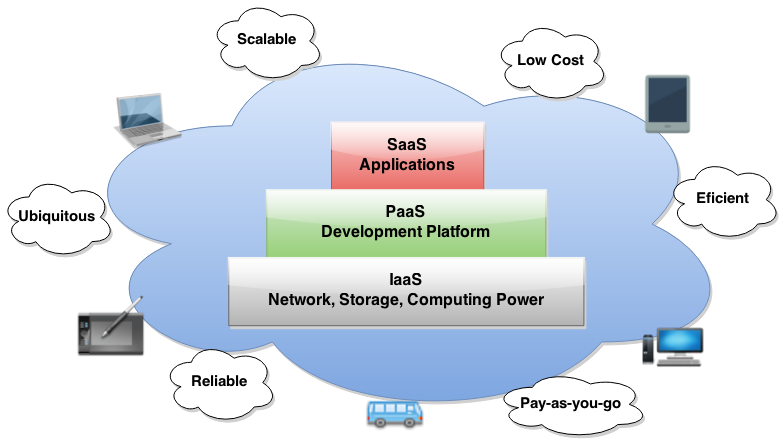
\includegraphics[scale=0.50]{Imagens/cap2_cloudremark.png}
    \caption{Diagram of Cloud Computing.}
    \label{fig:smart}
\end{figure}

The cloud is reliable in that it provides access to applications and documents anywhere in the world via the Internet. Cloud computing is often considered efficient because it allows organizations to free up resources and thus be able to focus on innovation and product development. 

For the purposes of this work, it is necessary to design and implement a cloud service for the proposed vehicular public safety application, as well as other areas that can make use of the information acquired by cloud. 

\section{Conclusion}

In this chapter, there has been a general overview of the technologies related to this work and its main concepts . In the next Chapter, there will be a detailed account of the "Related Works".